\documentclass[twocolumn,aps,pra,superscriptaddress,nofootinbib,longbibliography]{revtex4-2}
\usepackage{graphicx}% Include figure files
\usepackage{dcolumn}% Align table columns on decimal point
\usepackage{bm}% bold math
\usepackage[latin5]{inputenc}% For Turkish characters
\usepackage{amssymb}
\usepackage{amsmath}
\usepackage{amsthm}
\usepackage{amsbsy}
%\usepackage{mathptmx}
\usepackage{amsfonts}
\usepackage{mathtools}
\usepackage{physics}
\DeclareMathAlphabet{\mathcal}{OMS}{cmsy}{m}{n}
\usepackage{tabularx}
\usepackage{xcolor}
\usepackage{mathtools}
\usepackage{oubraces}
\usepackage{dsfont}
\usepackage[title, titletoc]{appendix}
\usepackage{graphicx}
\usepackage{rotating}
\usepackage[most]{tcolorbox}
\usepackage{enumerate}
\usepackage{subfloat}
%\usepackage{hyperref}% add hypertext capabilities
\usepackage[colorlinks=true,linkcolor=blue,citecolor=blue,urlcolor=blue]{hyperref}%
\usepackage{cleveref}
\usepackage[normalem]{ulem}
\Crefname{subfigures}{figure}{figures}
\Crefname{subfigures}{Figure}{Figures}


\newcommand{\tcr}[1]{{\color{red} #1}}
\newcommand{\tcb}[1]{{\color{blue} #1}}
\newcommand{\tcg}[1]{{\color{gray} #1}}
\newcommand{\vari}[1]{\text{Var}(#1)}


\def\bra#1{\mathinner{\langle{#1}|}}
\def\ket#1{\mathinner{|{#1}\rangle}}
%\def\braket#1{\langle{#1}|\rangle}
\def\Bra#1{\left<#1\right|}
\def\Ket#1{\left|#1\right>}
%\newcommand{\dd}{\differential}

%\newcommand{\nc}{\newcommand}
%\nc{\rnc}{\renewcommand}
%\nc{\beg}{\begin{equation}}
%\nc{\eeq}{{\end{equation}}}
%\nc{\beqa}{\begin{eqnarray}}
%\nc{\eeqa}{\end{eqnarray}}
%\nc{\lbar}[1]{\overline{#1}}
%\nc{\bra}[1]{\langle#1|}
%\nc{\ket}[1]{|#1\rangle}
%\nc{\ketbra}[2]{|#1\rangle\!\langle#2|}
%\nc{\braket}[2]{\langle#1|#2\rangle}
%\newcommand{\braandket}[3]{\langle #1|#2|#3\rangle}

\DeclarePairedDelimiter\ceil{\lceil}{\rceil}
\DeclarePairedDelimiter\floor{\lfloor}{\rfloor}

\newtheorem{theorem}{Theorem}
\newtheorem{lemma}[theorem]{Lemma}
\newtheorem{definition}[theorem]{Definition}
\newtheorem{corollary}[theorem]{Corollary}
\newtheorem{observation}[theorem]{Observation}
\newtheorem{proposition}[theorem]{Proposition}
\newenvironment{proof1}{\noindent\textbf{Proof:}}{\hfill \( \blacksquare \) \newline}



%***=============================================================***%
%***=============================================================***%


\begin{document}

\title{Deep Learning Project Progress Report}

\author{H\"useyin Talha \c{S}enya\c{s}a}
\email{senyasa@itu.edu.tr}
\affiliation{Department of Physics, Faculty of Science and Letters, Istanbul Technical University, 34469 Maslak, Istanbul, Turkey}




%\date{\today}

%***=============================================================***%
%***=============================================================***%

\begin{abstract}
My personal notes on \textit{An application of deep reinforcement learning to algorithmic trading}.

\end{abstract}

\maketitle

%***=============================================================***%
%***=============================================================***%


\section{Introduction}

\section{Implementation of the Framework}

In this section, we provide the details of the algorithmic trading framework. The framework consists of three main parts: Trading Environment, feed forward neural network and Double-Q mechanism. In this progress report, we provide the full detail of the trading environment which the RL agent interacts with, and then briefly report general structure of the remaining parts which are going to be implemented as a next step. 
 

\subsection{Trading Environment}

The nature of an environment in deep reinforcement learning applications is dictated by the problem in question. Although a trading action can be realized in a continuos medium i.e., a trading decision can be made at any time, algorithmic trading actions occurs in a discrete medium due to nature of the data to be processed.  In our case, the medium of the environment consists of discrete time series which is indexed by time step \(t\). The interval between sequential data points (corresponding to \(t-1\) and \(t\)) is determined by the trading frequency and it is denoted by \(\Delta t\). Since we only consider daily trading in this project, the interval \(\Delta t\) is equal to 1 day. 

\begin{figure}\label{fig:OHLCVfig}
    \centering
    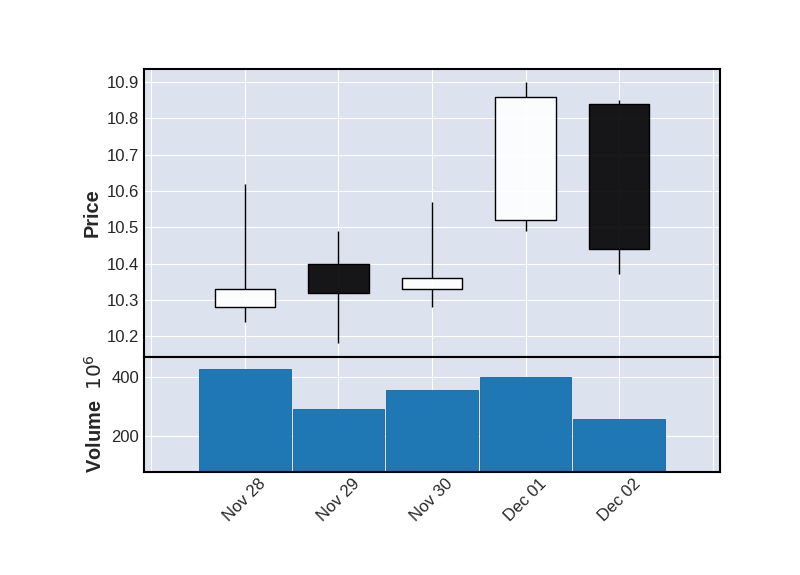
\includegraphics[scale=0.4]{Figs/Figures/OHLCV.png}
    \caption{A candlestick chart of \textit{Open, High, Low, Close}, for AAPL (Apple) stock with \textit{Volume} information. Here, a volume bar represents the total number of shares exchange during the corresponding interval.}
\end{figure}

The trading environment consists of three parts: Data retrieval, trading operations and RL agent interface. To be able to built the trading environment, one must first obtain the required data regarding the stock in question. Here, we use an open source third party \textit{Yahoo Finance} python interface to retrieve the classical OHLCV (\textit{Open, High, Low, Close, Volume}) data of the stock (for an example, see Fig.~\ref{fig:OHLCVfig}). Then one needs to implement trading operations (whose details is given in the next sub-section) to be able to execute trading decisions. Finally, one needs to implement RL agent interface to train the deep neural network. 

The information that is available to the agent for observation consists of two parts. The first part is the classical OHLCV (\textit{Open, High, Low, Close, Volume}) data of the stock in question, and the second part is the trading position which is denoted by \(P\). 
Formally the discrete observation space that is available to the agent at time step \(t\) can be expressed as 
\begin{equation}
    \mathcal{O}(t) = \{p_{t^{\prime}}^O, p_{t^{\prime}}^H, p_{t^{\prime}}^L, p_{t^{\prime}}^C, V_{t^{\prime}}, P_{t^{\prime}}\}_{t^{\prime} = t}^{t + \tau},
\end{equation}
where 
\begin{enumerate}[-]
    \item \(p_t^O\) is the opening price of the stock over the period \([t - \Delta t, t]\),
    \item \(p_t^H\) is the highest price over the period \([t - \Delta t, t]\),
    \item \(p_t^H\) is the lowest price over the period \([t - \Delta t, t]\),
    \item \(p_t^C\) is the closing price over the period \([t - \Delta t, t]\),
    \item \(V_t\) is the total volume of shares exchange over the period \([t - \Delta t, t]\),
\end{enumerate}
and \(\tau\) is called the \textit{state length} which is a hyper-parameter of the network. 

\subsubsection{Description of Trading Operations / Action Space}
Trading operations correspond to the actions that are available to the RL agent. The agent can buy or sell shares of the stock which translates into \textit{going long} and \textit{going short} respectively.  However, the RL agent must also decide the amount of shares it is going to buy or sell for a given time step \(t\) based on its portfolio e.g., \textit{cash} and \textit{number of shares}. To formally express the operations, we first define various quantities. Let \(C_{t} \in \mathds{R}^{\geq 0}\) be the available amount of cash at time step \(t\) and then let \(Q_t \in \mathds{R}\) be the number of shares exchanged at time step \(t\). Positive values of \(Q_t\) means that the agent buys shares i.e., \textit{taking long action}, on the other hand, negative values of \(Q_t\) means selling shares i.e., \textit{taking short action} while \(Q_t = 0\) corresponds to holding position. However, during the implementation of the agent, we eliminate \(Q_t = 0\) case (that is, the agent only decides to buy or sell), by handling the position transition in a way that the same sequential action corresponds to \textit{hold} position. Therefore, the complete action space over all time steps \(t\) can be defined as
\begin{equation}
    \mathcal{A}_t = \{Q^{\text{Long}}_{t}, Q^{\text{Short}}_{t} \,| \, t \in [t_i, t_f]\}.
\end{equation}
where \(t_i\) and \(t_f\) are initial and final trading days respectively.


The agent starts its trading activity with an initial \(C_{t=t_i}\) amount of money and it is chosen in such a way that it is much lower than the average exchange volume of the stock in question. In this way, it becomes safe to assume that the trading actions carried out by the agent does not influence the stock movements. At a time step \(t\), the agent takes an action \(a_t \in \mathcal{A}_t\) which effects the portfolio, that is, it effects the available cash \(C_t\) and the number of shares \(n_t\) owned by the agent. Their update rules are defined as
\begin{equation}\label{eq:portfolio-update}
    C_{t+1} = C_t - Q_t p_{t}^{c} - F \abs{Q_t} p_{t}^{c}
\end{equation}
where \(F\) denotes the trading cost. For a day trading, it is generally \(0.2\,\%\) of the exchange. We use this value as a trading cost.





Initialization, iteration and reset. In the initialization part, one first builds the environment in a state which can be determined randomly. This initialized state corresponds to current status of the environment. In the iteration part, first, the RL agent provides an \textit{action} to take, then, the environment state is transitioned to the next state according to the action provided by the RL agent.





% \begin{equation}
%     \begin{aligned}
%         \mathcal{E}_{TE} = \{&\text{Close, Low, High, Volume, Position,} \\
%         &\text{Action, Holdings, Cash, Money, Returns}\}
%     \end{aligned}
% \end{equation}

 








Let \(C_t\) be the available cash at time step \(t\) and let \(Q_t\) be the number of shares the agent is going to buy or sell. If the agent takes the long position at time step \(t\), the agent will have 
\begin{equation}
    Q_t = \floor*{\dfrac{C_{t}}{p_t^C (1 + T)}},
\end{equation} 


\subsubsection{Implementation of Trading Operations}



One first needs to implement the trading operations to be able to implement the trading environment. The trading operations correspond to the actions that is taken by the agent. In normal circumstances, there must be a match between bid and ask orders to realize a trade operation. In order to detect these matches, one must be able access the order book of the stock in question. However, since assume that the total number of buy and sell orders are much smaller than the volume of the stock, we are going to implement only buy and sell operations. 

The trading operations are implemented in an object oriented manner. There are two main classes to control trading operations: \textit{StockHandler} and \textit{DummyPosition}. The StockHandler class obtains the stock data and applies minor transformations to eliminate possible missing data points. This class also responsible for the real-time tracking of the stock via \textit{Update} method. The DummyPosition class is implemented to carry out possible actions i.e., \textit{long} or \textit{short} operations. and to keep track of the position changes. Here we provide the prototypes of the two classes. 


\subsubsection{Implementation of Trading Environment via OpenAI Gym}

The environment which the deep learning agent interacts with is implemented by utilizing \textit{OpenAI Gym} framework. OpenAI Gym is an open source python library that provides standardized application programming interface (API) to establish interaction/communication between agents and environments for reinforcement learning problems. 

A third party application has to implement/override several functions/methods that are inherited from the \textit{gym} base class. These methods include initialization, iteration and reset of the environment in question. 



\subsection{Implementation of Deep Neural Network}

Network Architecture, loss function etc.

\subsection{Implementation of Double-Q Mechanism}

\section{Additional notes and questions}

\begin{enumerate}
    \item Representing the transition from one candle to the next one as a Markov process.
    \item Considering the correlation between candles as a spin system (as in the case of Witten's ``An introduction to quantum information theory'') 
\end{enumerate}




\clearpage


\bibliography{biblio}

\end{document}

%%%%%%%%%%%%%%%%%%%%%%%%%%%%%%%%%%%%%%%%%%%%%%%%%%%%


% Some definitions and symbols

% \begin{enumerate}
%     \item \(S\): Set of environment and agent state.
%     \item \(A\): Set of actions which are available for agent to use.
%     \item \(s_t\): RL environment internal state
%     \item \(o_t\): Observation
%     \item \(a_t\): Trading action 
%     \item \(i_t\): Information
%     \item \(\pi(a_t|i_t)\): Trading policy (Rule)
%     \item \(r_t\): Network's reward.
%     \item \(\nu_{t}^c\): Total amount of cash in portfolio. 
%     \item \(\nu_{t}^s\): Corresponding value of the share.
%     \item \(n_t\): Total number of shares, lots. 
% \end{enumerate}

% Reinforcement learning techniques are concerned with the design of \(\pi\) maximizing an optimality criterion, which directly depends on the immediate rewards \(r_t\) observed over a certain time horizon. 